\section{Analysis}
\FloatBarrier % Now figures cannot float above section title

\subsection*{a}
Using the data in Table 2, the force vs deformation plot can be derived as \autoref{f3}. Also, from the lecture in week 7, we can learn that the total bending moment diagram is as follows


\begin{figure}[htbp]
    \centering
    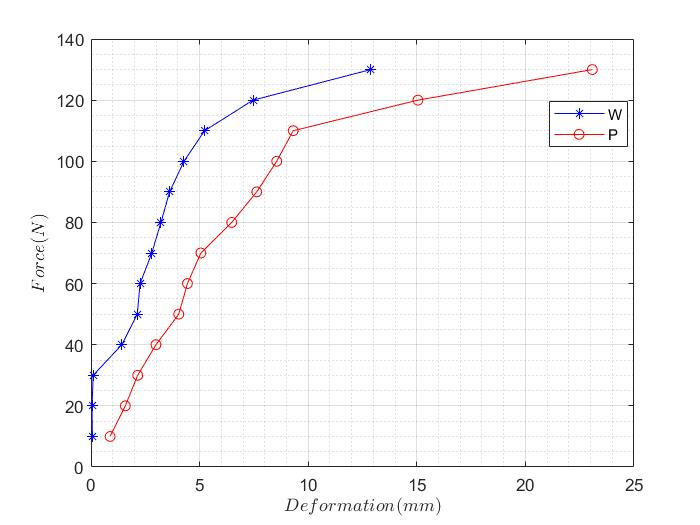
\includegraphics[width=9cm]{./fig/17.jpg}
    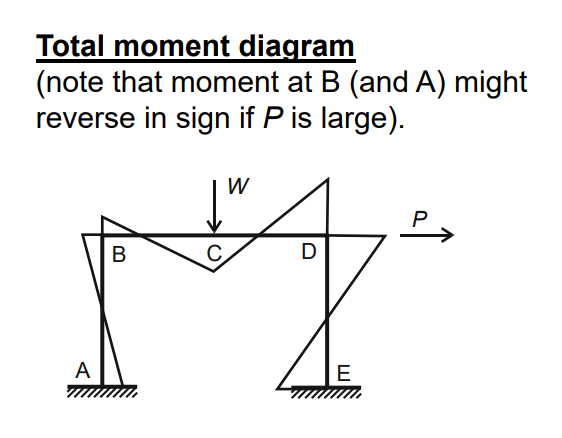
\includegraphics[width=7cm]{./fig/16.png}
    \caption{Force vs deformation and total moment diagram}
    \label{f3}
\end{figure}


The chart illustrates the relationship between the strength and deformation of steel, which can be discussed in two different situation.

$\bullet$ W<120N,P<110N: Elastic deformation: The relationship between the elastic deformation variable and the external force is linear.

$\bullet$ W$\geq$120N,P$\geq$110N: Plastic deformation: The relationship between force and deformation is nonlinear, i.e., the strain shows a rapid increase with the increase of stress.

From the total moment diagram (\autoref{f3}), it can be seen that the bending moment at point D is the largest, and this point will be the first point in the experiment to achieve plastic deformation.






\iffalse
\subsection*{Comparison of results}

By comparing the experimental data(See Table \ref{t3}) with the results of the ANSYS analysis(See Table \ref{t4}), 
it can be found that all six groups of data measured in the laboratory have 
larger deformation values than the ANSYS analysis. This is due to the fact 
that the modulus of elasticity of the laboratory material is 172.67GPa(Mild Steel) and 63.75GPa(Aluminium), 
both of which are smaller than the theoretical value of the material(210GPa and 71GPa).


In addition, the percentage deformation of mild steel is larger than 
that of aluminium 
(i.e. $\frac{\delta_{AN}-\delta_{FE}}{\delta_{FE}}*100\%$)
and this may also be due to the larger modulus of elasticity of mild steel.
Result shows in Table \ref{t5}.

\begin{minipage}[htbp]{\textwidth}
    \makeatletter\def\@captype{table}
    \centering
    \scalebox{1.1}{
    \begin{tabular}{lllll} 
        \hline
        Force  & Mild Steel(mm)  &Error(\%)  & Aluminium(mm) & Error(\%)   \\ \hline
        $P=50N$ & 0.0190  & 16.534 & 0.0363  & 11.219 \\
        $P=100N$ & 0.0381 & 16.539  & 0.0789 & 12.186\\
        $P=150N$ & 0.0571 & 16.537  & 0.1183 & 12.187\\
        Average &        &   16.54     &      &  11.86    \\ \hline          
    \end{tabular}} 

    \caption{Difference deformation in Mild Steel and Aluminium}
    \label{t5} 
\end{minipage}






\subsection*{Possible reasons in error analysis}
$\bullet$ Insufficient material purity or inhomogeneous density 
resulting in a modulus of elasticity less than the theoretical value.

$\bullet$ The memory effect of the metal caused by repeated use of the original 
experimental piece resulted in inaccurate deformation of the measurement.

$\bullet$ Errors caused by machines not being calibrated before measurement or 
by the machine's own measurement issues.

\subsection*{Experimental improvements and optimisation}

$\bullet$ Replacement of materials with new materials which are not affected by 
the memory effects.

$\bullet$ Choose higher purity and more homogeneous density with higher precision 
components for measurement.

$\bullet$ Change the machine and take several measurements to avoid experimental chance.
\fi